	\chapter{Theoretical Introduction}

	\section{Cosmic Rays}

	In the late eighteenth-century, it was of general knowledge that an electroscope\footnote{An \textbf{electroscope} is a device that produces an electric shock due to the cumulative effects of many rays.} slowly loses its charge despite the insulators. In the early twentieth century, many physicists began to investigate this issue. Radioactivity had just been discovered recently, and it was known that it could disintegrate air molecules into positive and negative ions, \textit{i.e.}, into ionized air, which conducts electricity. So, they thought that the slow loss of the electroscope was due to radioactive substances in the earth's crust.

In 1912, \textbf{Victor Francis Hess} jumped into a balloon and was raised up to 5000 m of altitude, where he observed that, the greater the height was, the greater the loss of his electroscope. \textbf{Hess} thought that the mysterious radiation, called \enquote{ultra sharp}, was coming from outside the Earth and was attenuated as it crossed the atmosphere.

\textbf{Robert Andrew Millikan} was the one who in 1927 baptised this radiation with the name \enquote{Cosmic Rays}, thus beginning the boom of their study, aimed at deciphering their nature. This led to the invention of the \textit{Geiger-M{\"u}ller} counter in 1928, which was used for this study, replacing the electroscope, since it can detect each ray  separately. By 1930 the community started using the \textit{cloud chamber} and finally the \textit{photographic emulsion}.



	\section{Nature}

	In studies carried out until 1930, it was discovered that this radiation contains known rays ($\gamma$, X, $e^-$ $\dots$) going at high speed and great energy, as well as other new rays. The experiments revealed a wealth of new particles and high energies, from 1 to 1000 GeV and even $10^{19}$ eV. 

In one particular case, in 1991, the \enquote{\textit{Fly's Eye}}\footnote{Small detectors, each covering a small solid angle, so that each detects only a few photons from the air showers.} observatory at Dugway (Utah) in the U.S. was able to detect particles with energies around 300\e{18} eV, the highest ever recorded energy at the time, equivalent to about 20 J, which would be sufficient to raise 10 $^{\circ}$C the temperature of a tablespoon of water. This energy amounts to $\sim 10^9$ times greater than that achieved so far in manmade accelerators.

We have written this energy as a multiple of $10^{18}$ on purpose, since an energy of $10^{18}$ eV is what is known as the \textbf{Greisen--Zatsepin--Kuzmin barrier}, over which rays can interact with the gammas of background radiation, the Big Bang echo that might have occurred 15\e{9} years ago. It is known that above 7\e{18} eV, $\gamma$ radiation decays, perhaps due to such interaction.

As for particles with energies of 300\e{18} eV mentioned above, they would be less than 100\e{6} years old, so they would not have anything to do with the Big Bang, but could also come from a distant source which were less than 10\e{6} light years from Earth (see \cite{bir:95} for a detailed report on this event and \cite{hal:98} for a review of the highest energy cosmic rays and other references).

	\section{Classification}

	Cosmic radiation is classified in various ways, according to their energy or nature. On the energy side, we can divide it into PRIMARY radiation, which consists mostly of high-energy protons and SECONDARY radiation, which refers to the particle cascades produced by the primary.

According to their nature, they were classified, a bit empirically and a bit following tradition, into HARD and SOFT components, although physicist Werner K. Hei\ss enberg made ​​another classification into four components as follows:

\ben
	\item Soft, composed by $\gamma$ and $e^-$ whose total absorption is achieved with 12 cm. of Lead.
	\item Soft, produced by percussive processes of mesons and their decays.
	\item Hard or penetrating, which is made of fast mesons of different spins and half-lives in the atmosphere produced by the primary proton component. It can contain:
	\item p, n, $\nu$, $\gamma$ and nuclear fragments. This component's intensity continuously decreases at a slower rate than the soft component.
\een

	\section{Showers and cascades}

	Most rays of the atmosphere are secondary radiation. They were discovered by physicist \textbf{Pierre Auger} in 1938. The \enquote{Auger effect} is the emission of an $e^-$ from the extra-nuclear portion of an excited atom when the atom undergoes a transition to a state with a lower excitation energy. It is believed that a human is traversed 20 times per second by showers, causing secondary cascades in bones and tissues.

	\subsection{Latitude effect}

	\bfi[H]		
		\begin{minipage}[s]{0.3\textwidth} 
	    	\bc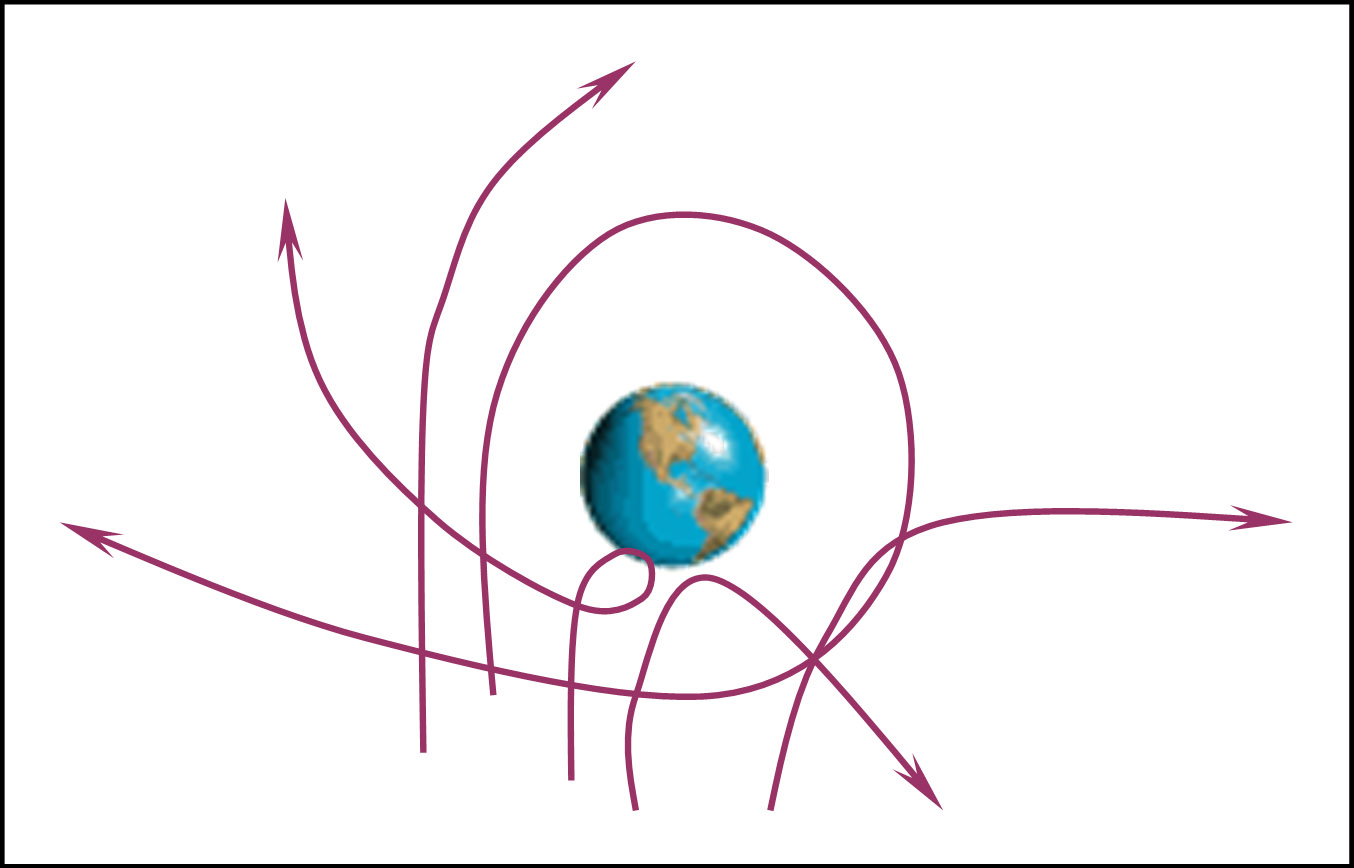
\includegraphics[width=\textwidth]{img/earth.jpg}\ec
		\end{minipage}
		\begin{minipage}[s]{0.7\textwidth} 
      		\captionsetup{width=0.8\textwidth}
			\caption[Earth, viewed from the North Pole.]{Earth, viewed from the North Pole. Effect of the magnetic field of the Earth in the equator on the trajectories of the primary cosmic rays.}\label{fig:earth}
		\end{minipage}
	\efi\captionsetup{width=0.8\textwidth}


	If we were able to study the properties of the primary radiation, it was thanks to the Earth's magnetic field, which bends the trajectories of charged secondary particles. This \enquote{magnetic barrier} is more effective near the equator, and gradually decreases with increasing altitude. Since primary cosmic rays are charged, they (and the secondary) should be more abundant at higher latitudes. This phenomenon is called the \textbf{latitude effect} and led to the discovery that primary rays are charged.

The theory also proves that the positive particles are deflected such that they arrive preferably from Western directions, and negative charged ones from the East. Since the measurements returned higher intensities in the western than in the eastern direction, it follows that the primary particles are mostly positive. So \textit{\textbf{the cosmic radiation varies with latitude and altitude and has an east-west asymmetry}}.


	\subsection{Secondary production process}

	As seen in \ref{fig:earth}, when a primary enters the atmosphere, it collides with an atom, which then decays into secondary cosmic rays, which in turn will decay or continue their path until colliding with another atom.

	Muons are known to be produced by pion decay according to different reactions:

\bc
	\graybox{.4}{.3}{
		$\pi^+ \rightarrow \mu^+ + \nu_\mu$\\
		$\mu^+ \rightarrow e^+ + \nu_\mu + \bar{\nu_e}$
	}

	\graybox{.4}{.3}{
		$\pi^- \rightarrow \mu^- + \nu_\mu$\\
		$\mu^- \rightarrow e^- + \bar{\nu_\mu} + \nu_e$
	}
	\graybox{.4}{.3}{
		{$\pi^0 \rightarrow \gamma + \gamma$}
	}
\ec

	Muons generally do not interact with the atomic nuclei ,and cross the atmosphere (losing about 2 GeV  \cite{eid:04}) until they sink into the earth or disintegrate into electrons. Meanwhile, while $\pi^0$ mesons and those with lower energy than the critical ($\epsilon_\pi$ = 115 GeV) decay immediately, the $\pi^+$ could even collide with other atoms. The phenomenon of \textbf{materialization} can also appear, when the $\gamma$ rays pass near the electric fields of nuclei and \textit{materialize} into electrons in accordance with the reaction: $\gamma \rightarrow e^+$ + $e^-$.

	All these reactions can be seen in Fig. \ref{fig:cascades}.

    \bfi[H]
      \bc
      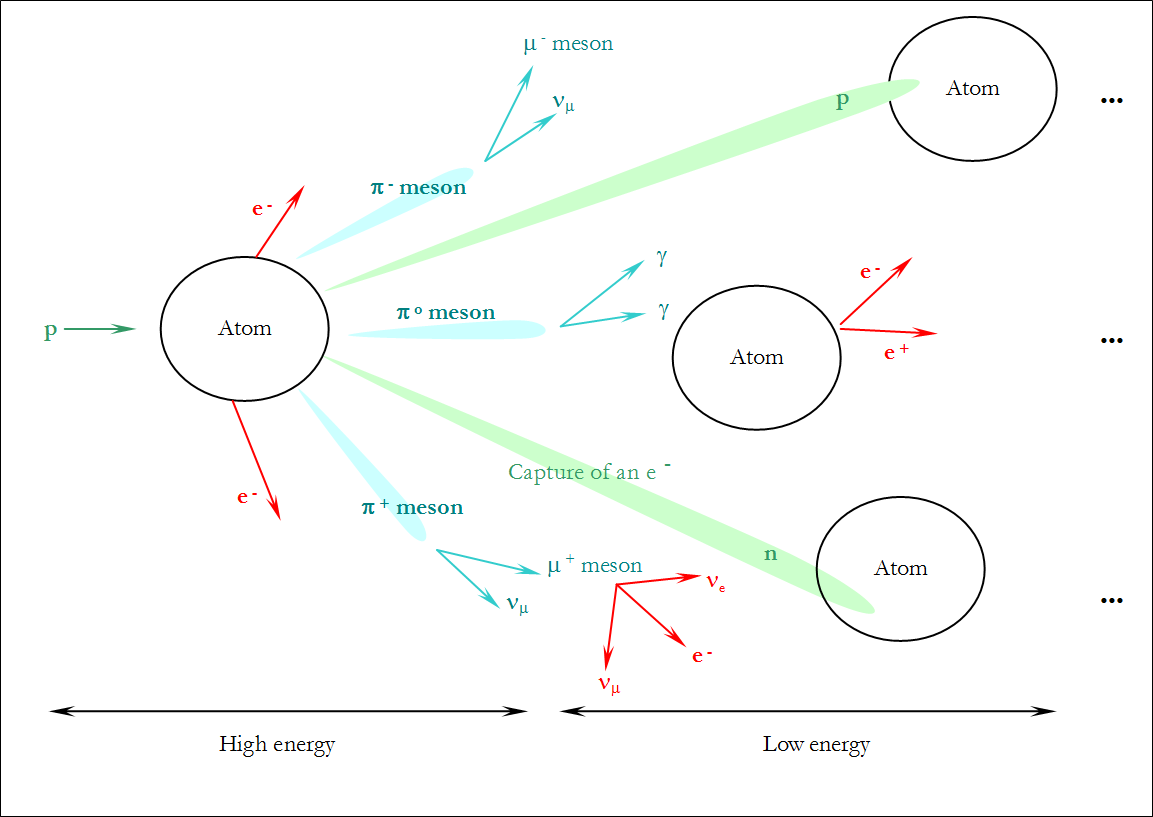
\includegraphics[width=14cm]{img/cascades.png}\\[12pt]
      \caption[Production of secondaries in Earth's atmosphere.]{Rough picture of the production of secondary in Earth's atmosphere, where the waterfall is produced by a 20 GeV proton at an altitude of 16 km.}\label{fig:cascades}
      \ec
    \efi


	All these particles from a cascade produced by a primary particle can reach the ground simultaneously, covering large hectares. Depending on the energy of these primary incident particles, more or less secondaries are produced:

	\bi
		\item If $E \geq 10^6$ GeV, $\sim 10^5$ secondary particles  are produced.
		\item If $E \geq 600\e{6}$ GeV, $\sim 10^8$ secondary particles are produced.
	\ei

These cascades can be described by a set of coupled equations and Monte Carlo simulations, but can also be approximated analytically in certain energy ranges. For example, the primary nucleons intensity per nucleon energy (E) in the energy range of GeV to $10^2$ TeV can be approximated by the expression:

	\be\label{eq:in} I_N(E) = 1.8 E^\alpha nucleon/ cm^2GeV\ee


where $\alpha$ is the differential spectral index of the cosmic-ray flux and has a value of 2.7.
Furthermore, the vertical intensity of nucleons after crossing an atmospheric thickness X in gcm$^{-2}$ is given by \cite{eid:04}:

	\be\label{eq:in2} I_N(E, X) \approx I_N (E, 0)e^{\frac{-X}{\Lambda}} \ee

where $\Lambda$ is the mass absorption coefficient that gives an idea of ​​the range of nucleons in air, while the corresponding expression for pions with energies much lower than the critical ($\epsilon_\pi$) is \cite{eid:04}:

	\be\label{eq:ipi} I_\pi(E_\pi, X) \approx \frac{Z_{N\pi}}{\lambda_N}I_N (E_\pi, 0)e^{\frac{-X}{\Lambda}}\frac{XE_\pi}{\epsilon_\pi}\ee


where the $Z_{N\pi}$ factor has to do with the distribution of charged pions in interactions of nucleons with nuclei of the atmosphere. This expression has a maximum at 15 Km of altitude.

In the case of the soft component, the most common electromagnetic cascades can be of two types, \textit{bremmstrahlung} and pair production.

However, at sea level, the most abundant secondary particles are muons. Energy and angular distribution are given by a convolution of the spectrum of production, energy loss into the atmosphere and the decay\footnote{For example, 2.4 GeV muons would travel 15 Km in the atmosphere before decaying, but this distance is reduced to 8.7 Km due to energy losses.}. Their average energy in the ground is about 4 GeV, for which the angular distribution is proportional to $cos^2\theta$.



	\section{Origin}

	Their origin is still being studied. Some observations:

	\bi
		\item The intensity of the cascades increases with solar perturbations, electromagnetic high frequency radiation emitted by the Sun contributes to the radiation reaching us. The remaining particles from outside the Solar System are modulated by the solar wind, which slows and excludes the rays of lower energy (<10 GeV) from the initial beam \cite{eid:04}.

		\item They are believed to be a remnant of some supernovae in our galaxy. However, higher energy rays would originate outside the Milky Way.

		\item It is thought that cosmic rays are trapped in the magnetic field of the galactic system for periods of 1 to several million years, causing energy densities $\sim$ 1 eV / cm$^3$ (approximately the energy of the magnetic field of the Sun). This capture increases radiation intensity, and explains why they arrive in equal numbers in all directions of the sky.

		\item The primary radiation is very different from what it was originally. Looking at Table \ref{tab:composition}, if we compare the composition of the radiation with the radiation of many stars, we see that is favoured in heavy elements and poor in the light ones, so they must have originated from the stars whose evolution is more advanced.
	\ei


    \ctable [
	cap     = {Composition of the Cosmic rays.},
 	caption = {Composition of the Cosmic rays.},
 	label   = {tab:composition},
	width   = 0.5\textwidth,
 	pos     = H,
	]
	{		r				D{.}{.}{5.4}      }{}
 	{\FL
         	H (p)			& 91.7\\
         	He ($\alpha$ particles)	& 7.6\\
         	Li, B, Be		& 0.13\\
         	C, N, O, F		& 0.35\\
         	Z > 10 			& 0.22
    \LL}

